\subsection{研究方案和技术路线}

\begin{figure}[h]
    \begin{small}
        \begin{center}
            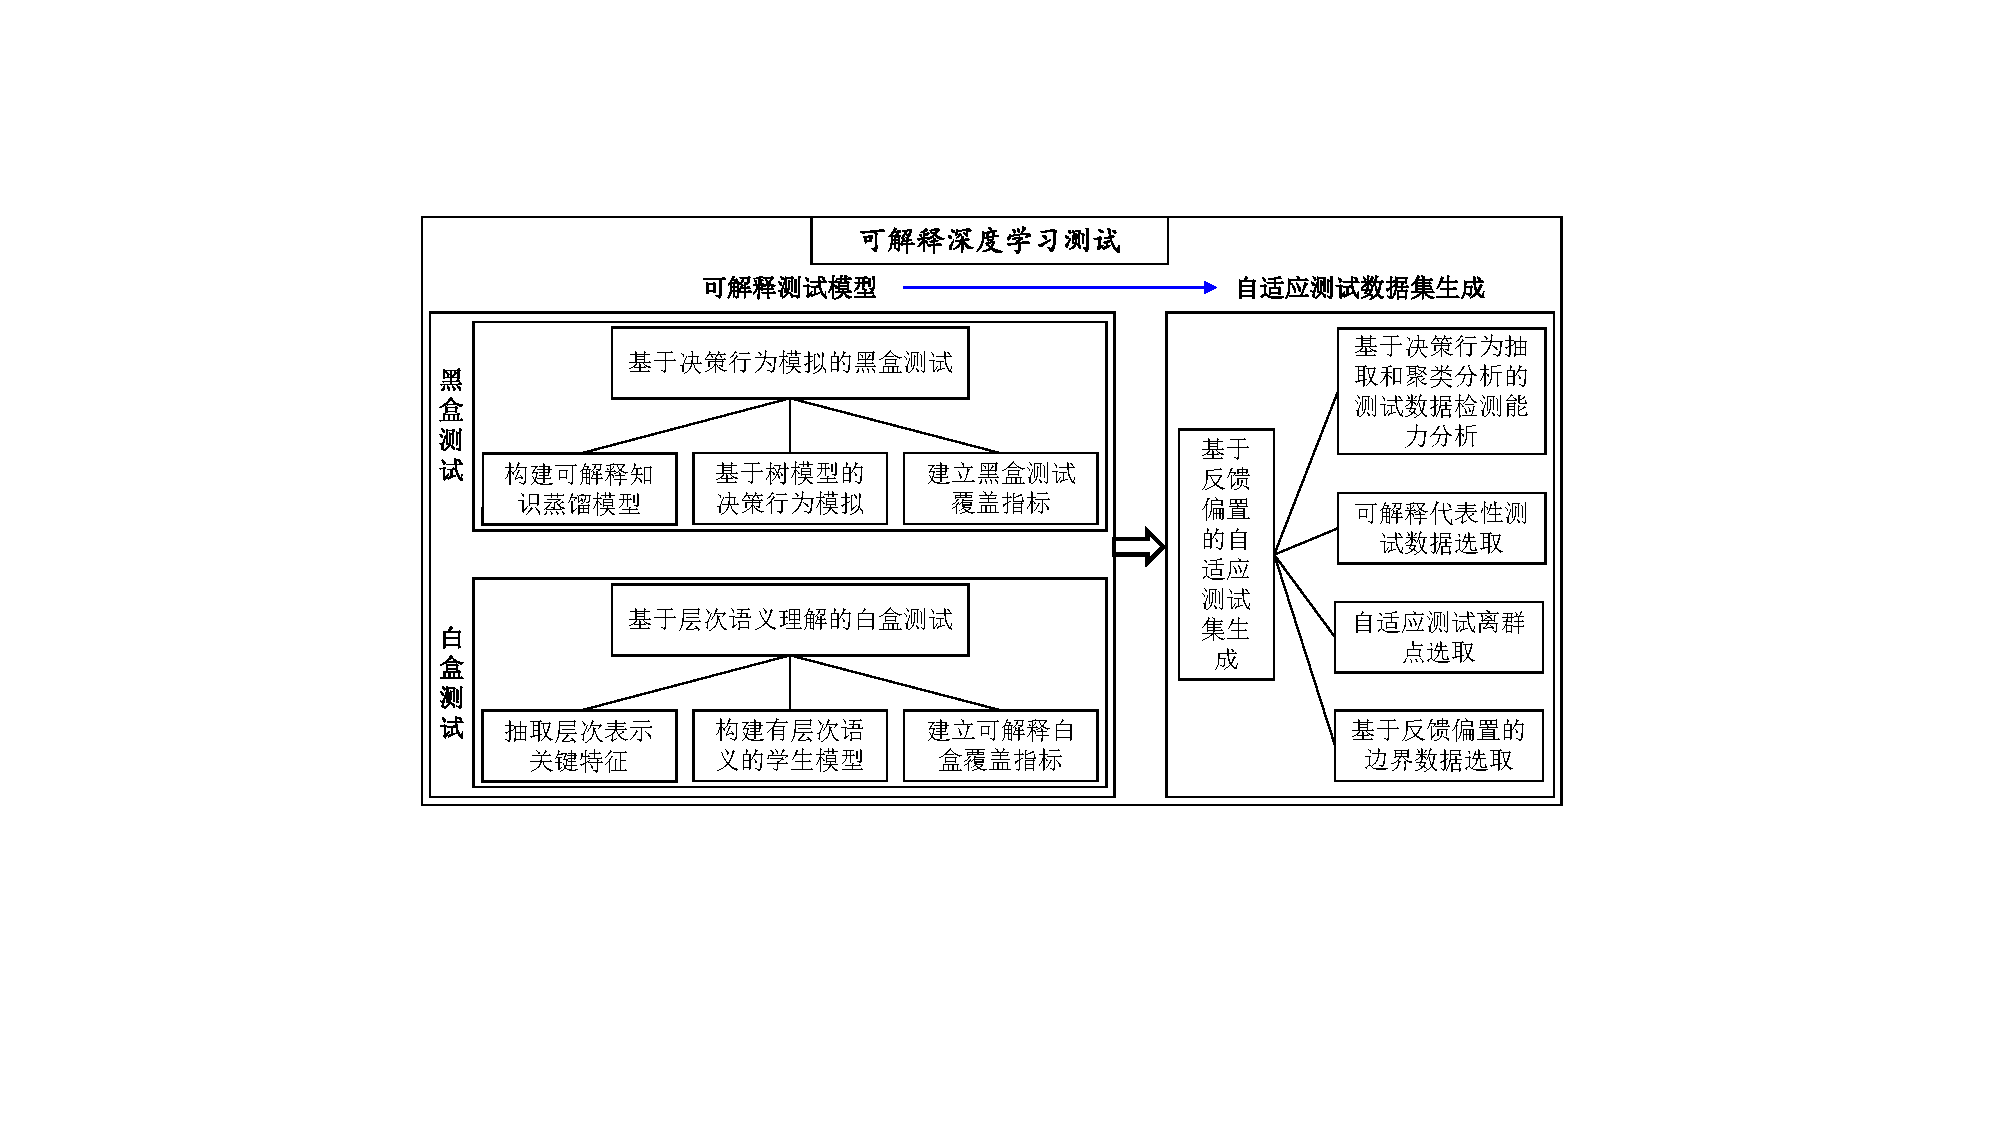
\includegraphics[width=0.95\textwidth]{ch3solution.pdf}
        \end{center}
        \caption{总体技术路线}
        \label{fig:ch3:solution}
    \end{small}
\end{figure}

围绕\ref{ch2content}规划的研究内容和\ref{ch2target}制定的研究目标,本项目拟定的
总体技术路线如\cref{fig:ch3:solution}所示。本项目针对大规模深度学习模型构建可解
释测试解决方案,从黑盒测试和白盒测试两个角度构建基于知识萃取的可解释蒸馏模型,分
别提出基于决策行为模拟的黑盒测试覆盖指标和基于层次语义理解的白盒测试覆盖指标,并
在此基础上实现基于反馈偏置的自适应测试集生成,通过基于实例的解释方法和自适应反馈
偏置分别选取代表数据和边界数据,实现具有可解释性和伸缩性的深度学习模型测试框架。



\subsubsection{基于决策行为模拟的黑盒测试}\label{ch3_1}

借鉴传统软件的路径覆盖测试方法,许多研究提出针对深度学习模型的覆盖性测试方法(参
见\ref{relatedwork} 国内外研究现状及发展动态分析),这些测试覆盖指标和方法主要是
针对白盒的场景,即测试者掌握所有的训练数据和整个深度学习模型,\textbf{但在许多场
景中,测试者无法访问训练数据和模型内部结构,但仍需要对模型的泛化能力进行测试,即
黑盒测试,如深度学习模型是某个公司私有的或者由第三方机构提供,他们只提供了接口或
者打包的可执行程序。}因此,本项目面向黑盒测试场景,研究基于决策行为模拟的黑盒测
试方法。

\cref{fig:ch3:2Btest}展示了本项目基于决策行为模拟的黑盒测试研究方法,如
图所示, \textbf{本项目拟利用知识蒸馏技术萃取黑盒模型中的知识}。就申请人所知,目
前尚未有基于知识蒸馏的深度学习覆盖度测试研究。首先,本项目利用知识蒸馏技术从黑盒
模型(``教师''模型)中萃取知识,训练一个小模型(``学生''模型)模拟其预测行为,在
知识蒸馏中,``教师''模型被视为黑盒模型,正好契合本项目黑盒测试的场景;其次,本项
目拟设计针对小模型的测试方法,间接评估黑盒模型的泛化能力,一方面,蒸馏得到的``学
生''模型复杂度低,可有效解决深度学习模型测试计算开销大的问题,另一方面,``学生''
模型的内部结构可以自定义,测试者也可访问,本项目拟利用基于树的模型(如:决策树、
随机森林等),以提高测试结果的可解释性。

具体地,给定一个黑盒模型$\mathcal M$,本项目将$\mathcal M$视为``教师''模型,假定
对于任意的输入$x^{(i)}$,测试者仅能得到$\mathcal M$对于该输入预测的概率分布,即
$x^{(i)}$属于各类的概率,记为$p^{(i)}$。$(x^{(i)}, p^{(i)})$的对应关系即为模型
$\mathcal M$中蕴含的知识,将作为训练``学生''模型时的软目标。\textbf{本项目拟构建
基于树的模型作为``学生''模型,记为$\mathcal M_t$,以支持可解释模型测试}。根据知
识蒸馏的思想,在训练``学生''模型时,本项目融合软目标$(x^{(i)}, p^{(i)})$和硬目标
$(x^{(i)}, y^{(i)})$构建``学生''模型的损失函数,使树型模型的输出同时接近黑盒模型
的概率分布$p^{(i)}$和真实标签$y^{(i)}$。值得注意的是,在训练``学生''模型时,直接
使用``教师''模型SoftMax层的输出结果$p^{(i)}$不合适,因为小模型无法直接学习得到大
模型的效果,我们通过在``学生''模型的损失函数中引入知识蒸馏中的T(Temperature)参
数,放大分类错误的误差,缩小正确分类的误差,可有效提高``学生''模型训练的效果。

\begin{figure}[htp]
    \begin{small}
        \begin{center}
            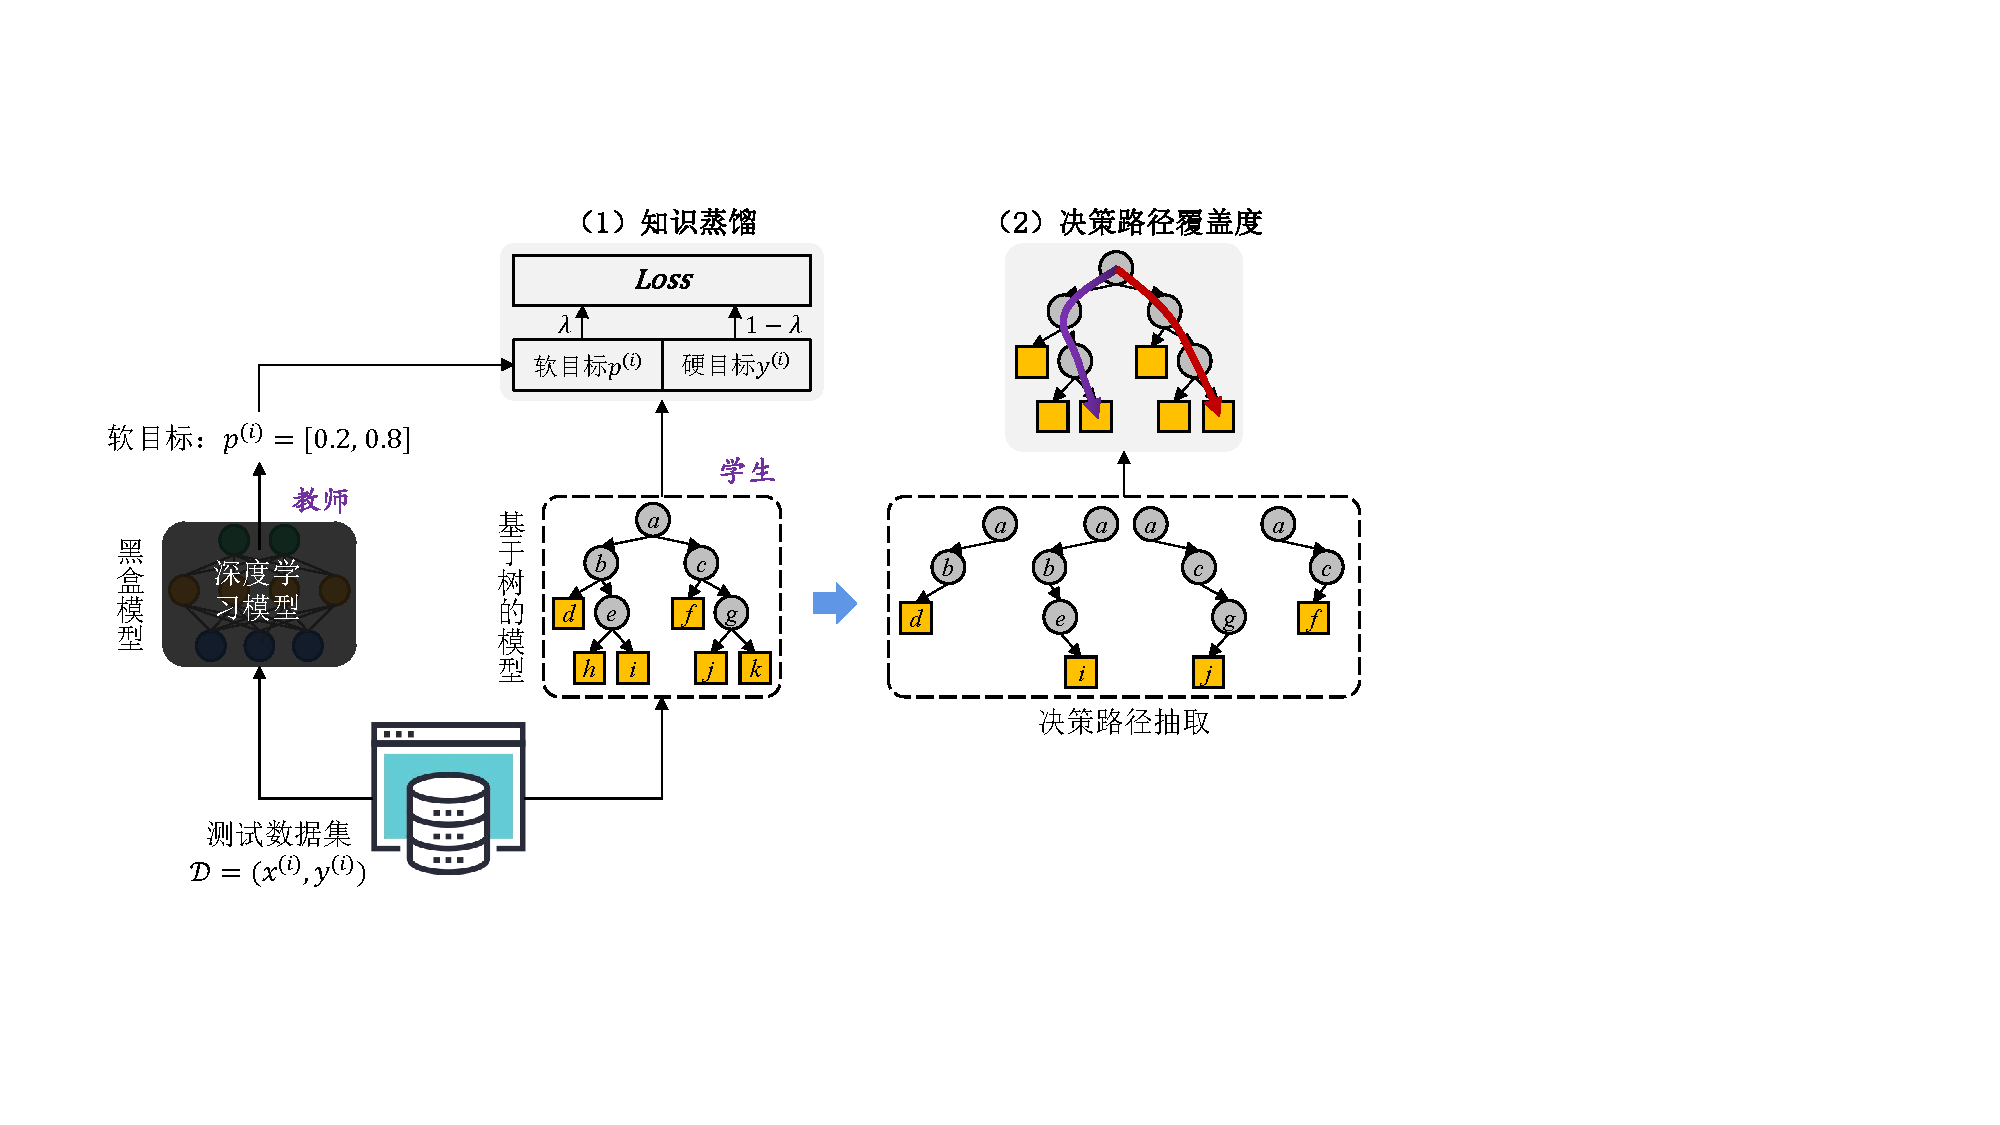
\includegraphics[width=0.9\textwidth]{ch3_2Btest.pdf}
        \end{center}
        \caption{基于决策行为模拟的黑盒测试研究方案}
        \label{fig:ch3:2Btest}
    \end{small}
\end{figure}


\textbf{本项目拟针对``学生''模型建立基于决策路径的覆盖性测试方法},知识蒸馏得到
的``学生''模型$\mathcal M_t$的预测行为非常接近原黑盒模型$\mathcal M$,针对
$\mathcal M_t$的覆盖度测试能比较准确地反映$\mathcal M$的泛化能力。首先,从基于树
的``学生''模型$\mathcal M_t$中抽取该模型对每个测试样本的决策路径,得到路径集合
$\mathcal P=\{t_1, t_2,\dots, t_l\}$,$l$表示路径数。然后,\textbf{本项目拟利用
统计方法建立基于决策路径的覆盖度指标},以评估测试用例集的充分性,其基本思想为对
树模型的决策路径覆盖度高的测试用例集具有良好的充分性,在此基础上,本项目拟计算决
策路径覆盖频率和正态分布的拟合程度来评估测试用例集的分布,可采用
Kolmogorov-Smirnov检验、D检验等方法,并结合正太性检验方法的拟合优度和决策路径的
覆盖度作为测试用例集充分性评价指标。此外,\textbf{本项目拟利用树模型的可解释性,
总结归纳模型错误行为的原因,指导训练数据集扩充和模型优化}。

\subsubsection{基于层次语义理解的白盒测试}\label{ch3_2}

本项目针对白盒测试的研究方案首先利用知识蒸馏技术,训练可解释的``学生''模型。以
\cref{fig:ch3:WBtestKD}为例,\textbf{本项目拟首先从给定的白盒模型中抽取其预测行
为},具体而言,本项目拟采线性判别分析(Linear Discriminative Analysis, LDA)抽取
各层样本表示的关键特征,同时可实现降维的效果,有效提高后续分析计算的效率,然后,
利用自底向上的层次聚类方法,对LDA得到的关键样本特征进行聚类,理清每一组神经网络
层的判别决策能力。本项目认为深度学习模型对输入的表示学习是一个从粗粒度到细粒度的
过程,因此,浅层表示(如第1组的输出)没有能力将样本分为最终指定的类别,仅能做到
粗粒度分类,但层次聚类算法会以打到最大类别数为目标,所以\textbf{本项目拟分析中间
层表示的整体分布,修改层次聚类的优化目标,或者在层次聚类之后,再合并相近的簇,以
准确反映中间层的决策语义}。

\begin{figure}[htp]
    \begin{small}
        \begin{center}
            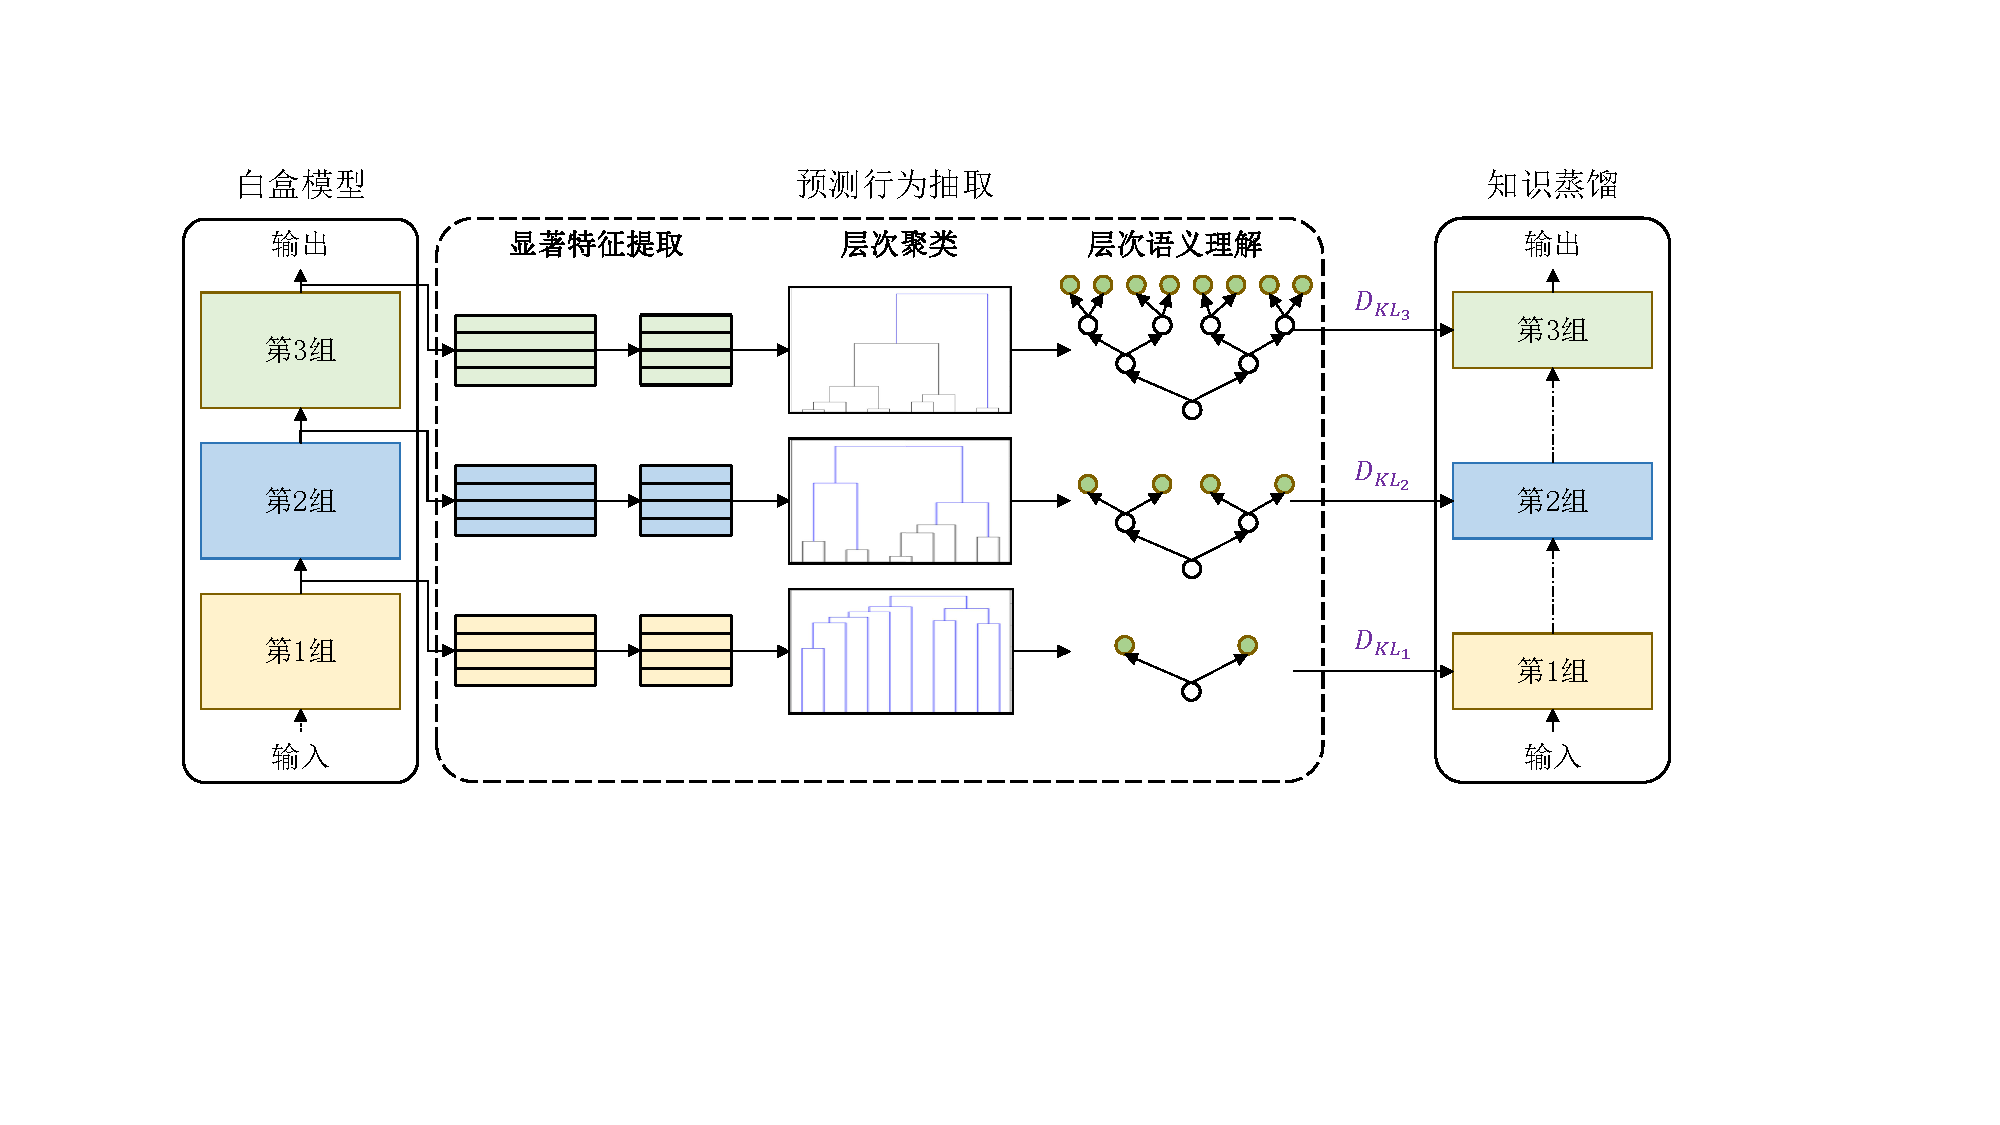
\includegraphics[width=0.95\textwidth]{ch3_WBtestKD.pdf}
        \end{center}
        \caption{基于层次语义理解的知识蒸馏研究方案}
        \label{fig:ch3:WBtestKD}
    \end{small}
\end{figure}

另一方面,\textbf{得到各组(层)的决策语义后,本项目拟改进知识蒸馏的方式,将各层
的决策语义融入``学生''模型的优化目标中},其主要思想如公式\eqref{eq:kd}所示:
\begin{equation}
    \mathcal{L} = \mathcal{L}_o + \beta\sum_{k=1}^L KL(p(f_s^k(\bm x_i)), p(g^k(y_i))) \,,
    \label{eq:kd}
\end{equation}
其中$\mathcal L_o$是``学生''模型原有的损失函数,$f_s^k(\bm x_i)$表示``学生''模型
第$k$层的表示向量,$g^k(y_i)$将数据标签$y_i$转换成第$k$层的语义标签,本项目拟用
KL散度来度量``学生''模型表示向量的分布是否和抽取的决策语义接近,作为损失函数的正
则项,引导``学生''模型训练。

得到可解释的``学生''模型后,本项目拟基于该模型提出决策路径覆盖度测试指标。根据公
式\eqref{eq:kd},在测试阶段,容易得到各层输出所属的粗粒度类别,\textbf{如
\cref{fig:ch3:WBtest}所示,本项目拟分析测试用例集对该决策路径图的覆盖程度,用以
评估测试用例集的充分性,同时,可检测``学生''模型针对某样本的分类过程是否有异常决
策路径(图中虚线所示),以分析模型在不同测试用例上的泛化能力},具有异常决策路径
的测试用例可能是边界样本,很可能引发模型错误,是模型进一步优化提供重要参考。
\begin{figure}[htp]
    \begin{small}
        \begin{center}
            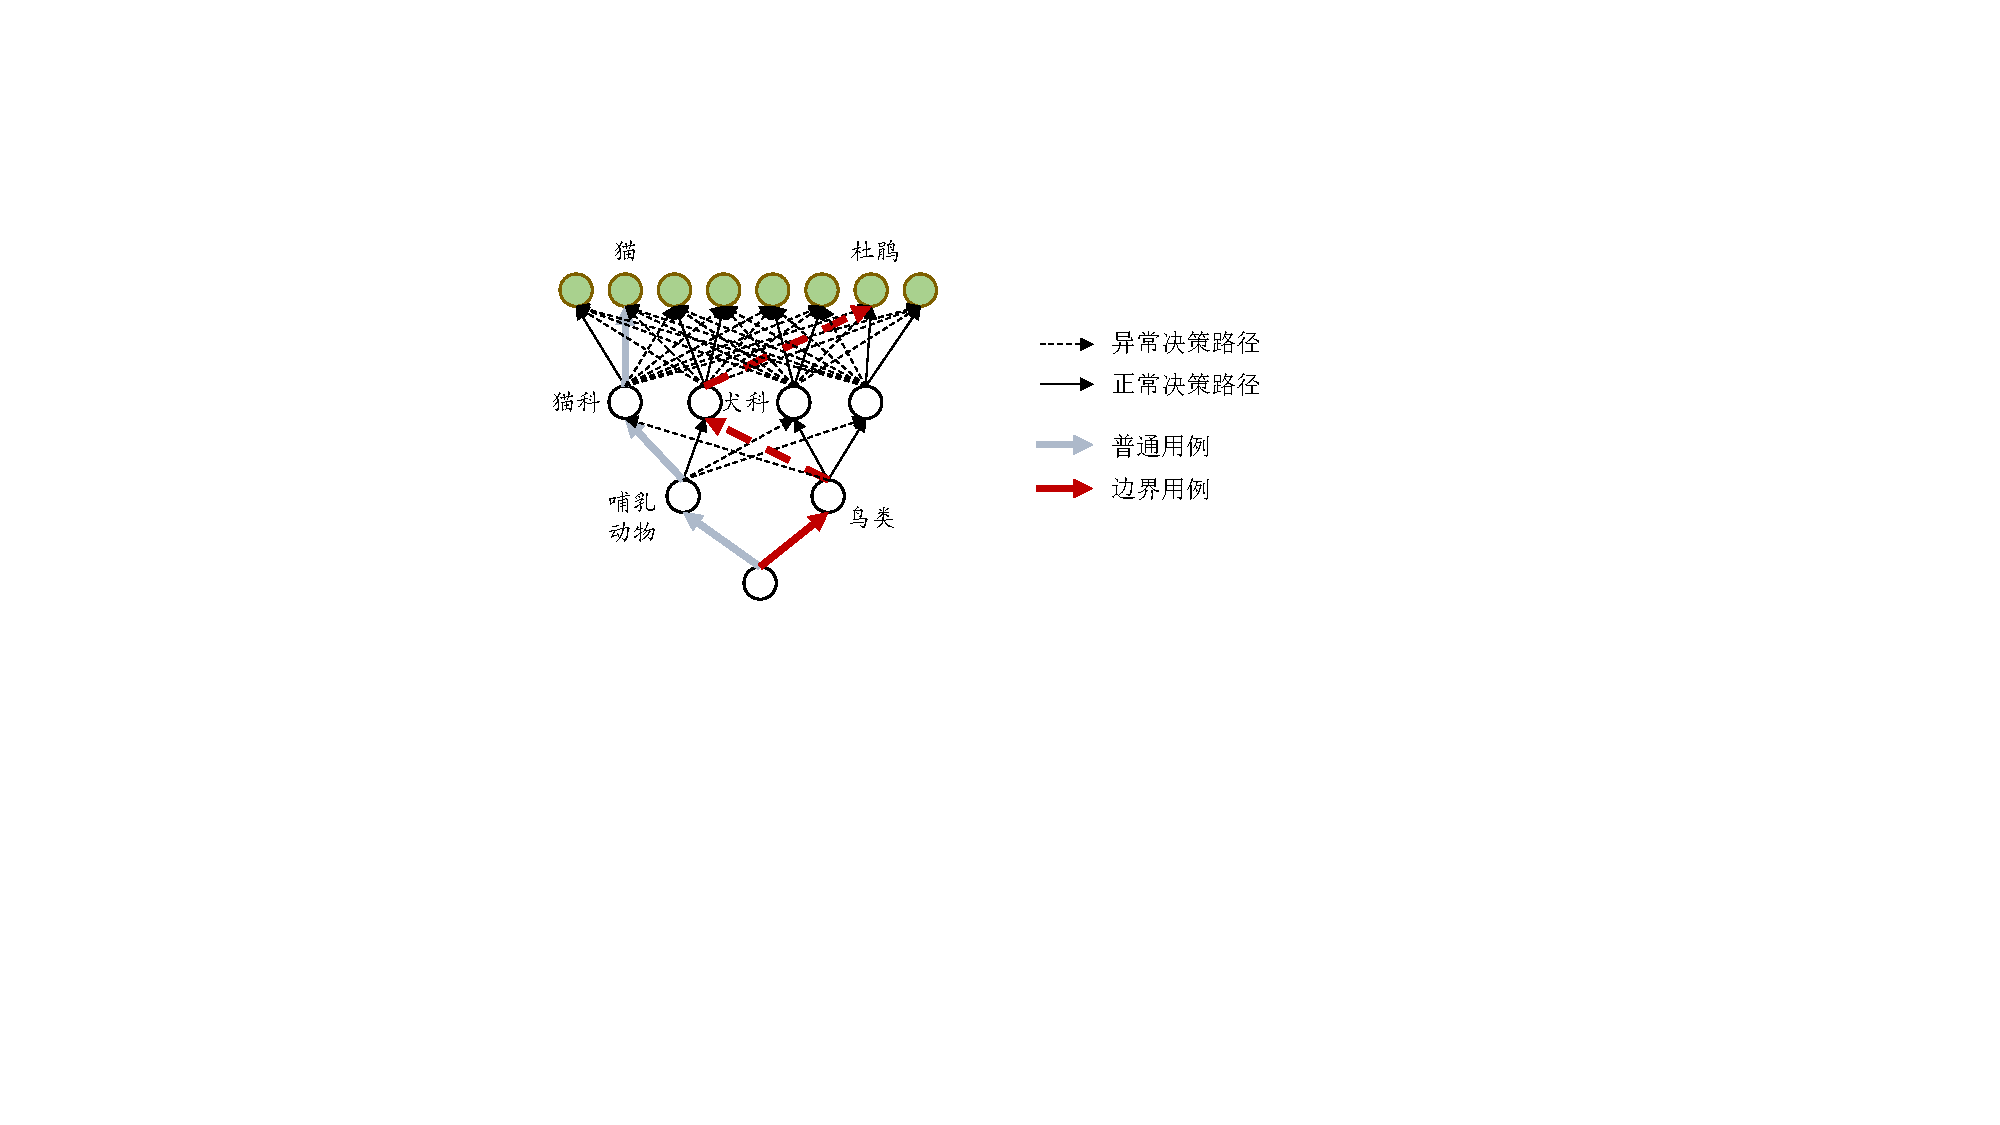
\includegraphics[width=0.65\textwidth]{ch3_WBtest.pdf}
        \end{center}
        \caption{基于可解释``学生''模型的覆盖度测试研究方案}
        \label{fig:ch3:WBtest}
    \end{small}
\end{figure}

\subsubsection{基于反馈偏置的自适应测试集生成}\label{ch3_3}

为了平衡测试集的规模和质量,针对给定大规模无标注数据,本项目拟在有限标注成本空间
内生成具有高代表性和检测能力的测试集,采用\textbf{基于实例的解释(Example-based
Explanation)}思想,选取代表性的样本来解释模型结果,得到与大规模无标注数据具有近
似决策路径分布的测试子集,估算模型性能。同时,为对深度学习模型进行充分性测试,本
项目\textbf{融合自适应测试和测试反馈},不断从离群点中选取与已选测试数据距离最大
的离群点,并根据与预测错误的测试数据相似性,尽可能找到导致模型错误行为的测试数据
优先标注。

%\textbf{聚类分析和最大平均差异法}( Maximum Mean Discrepancy,MMD)选取与大规模
%无标注测试数据具有近似决策路径分布的代表性数据作为测试集,并反馈已选测试数据及
%其测试结果反馈,自适应选择测试数据。基于实例的方法主要是通过一些代表性的样本来
%解释聚类/分类结果的方法


\begin{figure}[htp]
    \begin{small}
        \begin{center}
            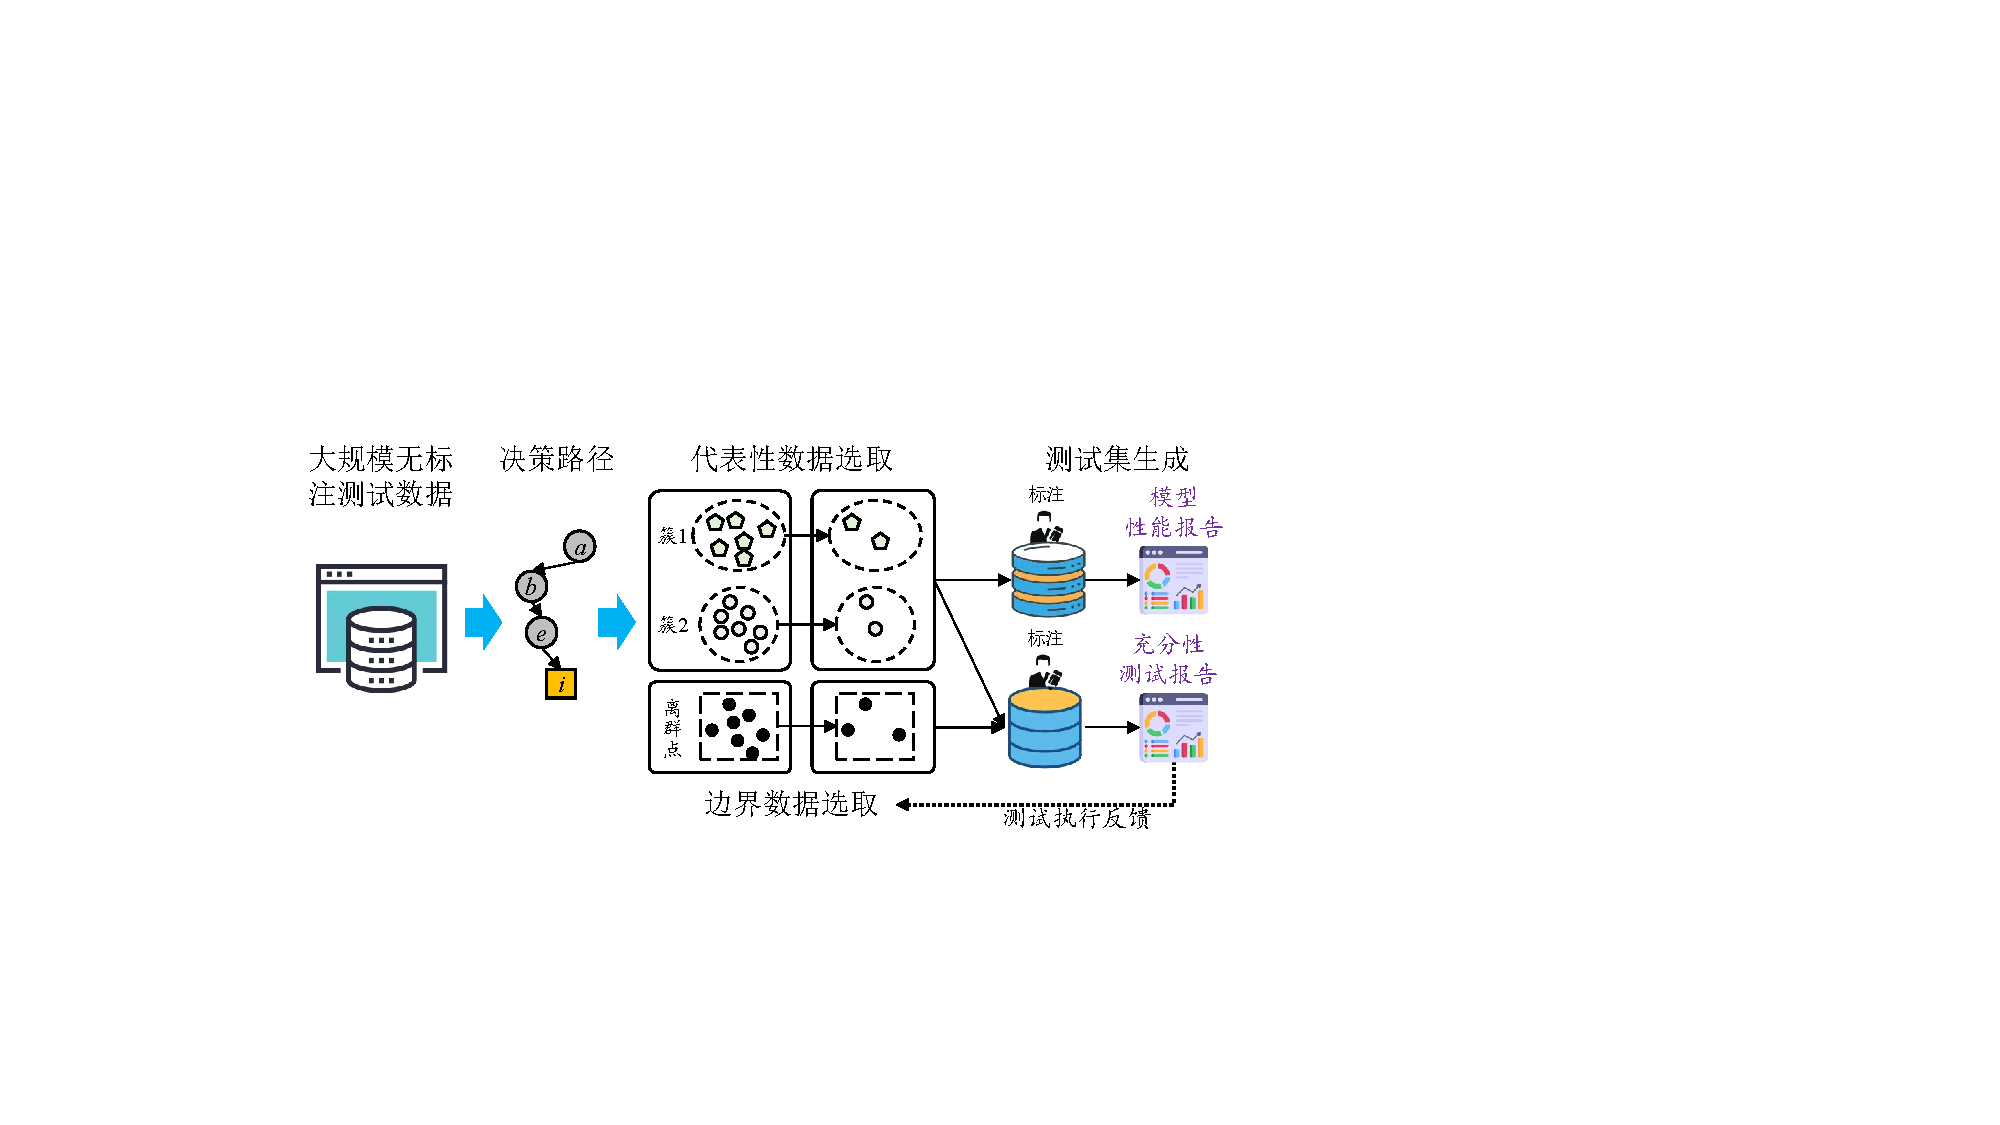
\includegraphics[width=0.85\textwidth]{ch3_TestSelection.pdf}
        \end{center}
        \caption{自适应测试集生成研究方案}
        \label{fig:ch3:interpretability}
    \end{small}
\end{figure}

\cref{fig:ch3:interpretability}是本项目针对深度学习模型自适应的测试集生成研究方
案示意图。为了提高可解释性和伸缩性,本项目在抽象可解释决策路径的基础上,结合决策
路径和聚类分析,区分具有不同检测能力的测试数据。以图中描述的模拟决策路径$t_i$为
例,每条决策路径对应的$n_i$个无标注测试数据为一组具有相似检测能力的测试数据。我
们对每组测试数据进行聚类分析,根据测试数据的规模大小将其聚为$k_i$类,将具有相同
决策路径的测试数据进一步划分为多簇。为了从大规模无标注数据中选取具有代表性的测试
数据,采用\textbf{最大平均差异算法}(Maximum Mean Discrepancy,MMD)从每类测试数
据中选取$m$个测试数据,若该类数少于$m$个则全部选取,构成初始测试子集。最大差异法
可表示为以下公式:
\begin{equation}
    \begin{aligned}
        \operatorname{MMD}(\mathcal{F}, P, Q)=\sup _{f \in \mathcal{F}}\left(\mathbb{E}_{X \sim P}[f(X)]-\mathbb{E}_{Y \sim Q}[f(Y)]\right)
    \end{aligned}
\end{equation}
其中$P$和$Q$分别为原测试数据分布和待选取测试数据分布,$\mathcal{F}$为再生西伯尔
空间,$\operatorname{MMD}(\mathcal{F}, P, Q)$用来衡量分布$P$和$Q$之间的距
离,\textbf{通过最小化MMD从每簇测试数据中选取具有解释性和代表性的测试数据,构成
代表性测试集},估算模型在大规模无标注数据上的性能。

为预防模型错误预测带来的损失,在测试覆盖指标和代表性测试集的基础上,进一步选择容
易导致错误行为的边界数据进行测试(见\cref{fig:ch3:interpretability})。在聚类分
析后,\textbf{采用自适应测试方法选取离群点,持续性选取与已选数据距离最大的测试数
据}进行充分性测试。同时,若经过标注和测试发现导致模型预测错误的测试数据,则
\textbf{将测试结果反馈到数据选择算子},选择与导致错误的测试数据具有相同决策路径
且在同簇中距离最近的测试数据进行充分性测试。

\subsection{可行性分析}

\subsubsection{理论可行性}

本项目研究目标明确,研究内容清晰,研究方案和技术路线中所应用的方法和技术手段在业
界都有着成熟清晰的理论基础。申请人和项目组对这些关键技术和理论有着深入的了解和掌
握,近年来在深度学习、软件测试、人工智能安全等领域的高水平会议上发表了多篇论文。
项目组前期已经对本项目中提到的研究内容分别进行了详细的调研和分析,并在深度学习白
盒测试、深度学习可解释性、软件质量和安全等领域取得了初步成果。因此,从理论上说,
本项目是可行的。

\subsubsection{技术可行性}

申请人前期调研了大量深度学习测试及其可解释性的研究工作(如\ref{relatedwork}节所
述),现有研究尚未形成可解释深度学习测试方法,主要受限于深度学习模型的规模太大、
可解释性差,而知识萃取方法可最大限度辅助模型理解,同时,最大平均差异法可以提供测
试数据选取的可解释性,因此,本项目利用知识萃取,构建基于路径的可解释覆盖测试指
标,并在此基础上,建立可解释数据选取方法,形成一套闭环深度学习测试框架,具有较强
的技术可行性。申请人之前的研究工作一直聚焦于深度学习测试和可解释性,在深度学习白
盒测试、模型可解释性和软件质量维护等方面已取得一定的研究成果,并在攻读博士期间主
导研发过开源工具。申请人所在项目组一直活跃在深度学习测试、软件安全、模型和数据安
全等相关领域,有着丰富的研究经验和技术积累。同时,在研究过程中,申请人与自动驾驶
公司(国汽智控)建立了合作关系,积累了大量可用于实验的真实数据集。因此,从技术上
说,本项目是可行的。

\iffalse
\subsubsection{团队合理性}

项目组在深度学习测试和模型安全具有一定的基础,积累了丰富的研究经验,在重要国际会
议上发表了多篇高水平论文,项目在开源软件开发和管理等方面也有丰富的积累,可为本项
目测试框架研发和开源推广提供保障。项目组梯队完善,队伍具有凝聚力和创造力,项目组
成员每周定期讨论,有着良好的科研氛围,同时对本项目的研究内容具有浓厚的研究兴趣。
申请人有着长期广泛的国内外合作者,申请人与合作导师Hua Ji教授,本学院的刘哲理教
授、范玲玲副教授,天津大学的陈森副教授等均有密切合作,他们一直活跃在软件测试、软
件安全和模型安全等领域的学术前沿,可为本项目提供技术指导。此外,申请人与联合培养
时的导师新加坡国立大学教授Siau-Cheng Kho一直保持密切联系,Kho教授长期从事软件安
全和深度学习方面的研究,是软件工程和软件安全方面非常活跃的科学家;申请人与新加坡
南洋理工大学教授Yang Liu合作密切,Liu教授在软件工程、开源软件分析域管理等方面有
着丰富且深入的研究,是相关领域的引领者。两位国际知名专家可为本项目提供技术指导。
\fi